\documentclass{standalone}
\usepackage{tikz}

\begin{document}

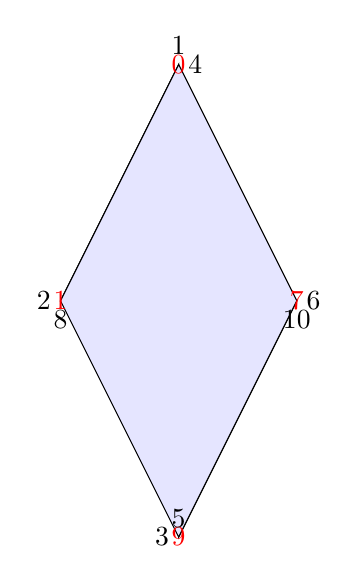
\begin{tikzpicture}[scale=1.5]
    % Define coordinates
    \coordinate (A) at (0, 2);
    \coordinate (B) at (-1, 0);
    \coordinate (C) at (1, 0);
    \coordinate (D) at (0, -2);

    % Draw the main diamond shape
    \draw[fill=blue!30] (A) -- (B) -- (C) -- (D) -- cycle;

    % Draw the inner diamond shape
    \draw[fill=blue!10] (B) -- (A) -- (C) -- (D) -- cycle;

    % Label the vertices
    \node[red] at (A) {0};
    \node[red] at (B) {1};
    \node[red] at (C) {7};
    \node[red] at (D) {9};

    \node at (B) [left] {2};
    \node at (C) [right] {6};
    \node at (D) [left] {3};
    \node at (A) [right] {4};

    \node at (B) [below] {8};
    \node at (C) [below] {10};
    \node at (D) [above] {5};
    \node at (A) [above] {1};
\end{tikzpicture}

\end{document}